\documentclass[12pt,a4paper]{article}\usepackage[]{graphicx}\usepackage[]{color}
% maxwidth is the original width if it is less than linewidth
% otherwise use linewidth (to make sure the graphics do not exceed the margin)
\makeatletter
\def\maxwidth{ %
  \ifdim\Gin@nat@width>\linewidth
    \linewidth
  \else
    \Gin@nat@width
  \fi
}
\makeatother

\definecolor{fgcolor}{rgb}{0.345, 0.345, 0.345}
\newcommand{\hlnum}[1]{\textcolor[rgb]{0.686,0.059,0.569}{#1}}%
\newcommand{\hlstr}[1]{\textcolor[rgb]{0.192,0.494,0.8}{#1}}%
\newcommand{\hlcom}[1]{\textcolor[rgb]{0.678,0.584,0.686}{\textit{#1}}}%
\newcommand{\hlopt}[1]{\textcolor[rgb]{0,0,0}{#1}}%
\newcommand{\hlstd}[1]{\textcolor[rgb]{0.345,0.345,0.345}{#1}}%
\newcommand{\hlkwa}[1]{\textcolor[rgb]{0.161,0.373,0.58}{\textbf{#1}}}%
\newcommand{\hlkwb}[1]{\textcolor[rgb]{0.69,0.353,0.396}{#1}}%
\newcommand{\hlkwc}[1]{\textcolor[rgb]{0.333,0.667,0.333}{#1}}%
\newcommand{\hlkwd}[1]{\textcolor[rgb]{0.737,0.353,0.396}{\textbf{#1}}}%
\let\hlipl\hlkwb

\usepackage{framed}
\makeatletter
\newenvironment{kframe}{%
 \def\at@end@of@kframe{}%
 \ifinner\ifhmode%
  \def\at@end@of@kframe{\end{minipage}}%
  \begin{minipage}{\columnwidth}%
 \fi\fi%
 \def\FrameCommand##1{\hskip\@totalleftmargin \hskip-\fboxsep
 \colorbox{shadecolor}{##1}\hskip-\fboxsep
     % There is no \\@totalrightmargin, so:
     \hskip-\linewidth \hskip-\@totalleftmargin \hskip\columnwidth}%
 \MakeFramed {\advance\hsize-\width
   \@totalleftmargin\z@ \linewidth\hsize
   \@setminipage}}%
 {\par\unskip\endMakeFramed%
 \at@end@of@kframe}
\makeatother

\definecolor{shadecolor}{rgb}{.97, .97, .97}
\definecolor{messagecolor}{rgb}{0, 0, 0}
\definecolor{warningcolor}{rgb}{1, 0, 1}
\definecolor{errorcolor}{rgb}{1, 0, 0}
\newenvironment{knitrout}{}{} % an empty environment to be redefined in TeX

\usepackage{alltt}
\usepackage[utf8]{inputenc}
\usepackage[T1]{fontenc}
\usepackage{polski}
\usepackage{enumitem}
\usepackage{amssymb}
\usepackage{lipsum} 
\usepackage{titling}
\author{Marcin Miśkiewicz, Adrian Sobczak}
\title{\textbf{Analiza podstawowych statystyk meczowych zawodników ligi NBA}}
\date{\today}
\IfFileExists{upquote.sty}{\usepackage{upquote}}{}
\begin{document}







\maketitle
\section{Wprowadzenie}

Odkąd profesjonalne organizacje sportowe zaczęły zatrudniać na pełen etat analityków i statystyków, charakter całych dyscyplin uległ pewnego rodzaju rewolucji. Specjaliści od danych z miejsca stali się bezpośrednimi doradcami kadry trenerskiej, a wyniki ich prac wprowadziły nowe trendy w sposobach treningu i samej gry. Dzisiaj system szkolenia oparty jedynie na solidnym przygotowaniu fizycznym ustępuje miejsca podejściu strategicznemu, mającemu w arsenale analizy wideo, pomiary wydolnościowe czy taktyki wyliczone pod konkretnych rywali. Jako kolebkę wdrażania zaawansowanej statystyki do sportu powszechnie uznaje się najsilniejszą ligę koszykarską na świecie --- NBA (\emph{National Basketball Association}). Dopiero amerykańscy pionierzy zainspirowali nowym sposobem myślenia działaczy z innych dyscyplin, takich jak piłka nożna czy siatkówka.

\section{Cel pracy}

Mimo że wewnętrzne statystyki klubów NBA są ściśle chronione, istnieją również powszechne bazy danych gromadzące szereg informacji na temat konkretnych zawodników. W niniejszej pracy wykorzystamy jeden z takich zbiorów i na jego podstawie wysuniemy garść wniosków m.in na temat panujących trendów w lidze, czy zależności pomiędzy poszczególnymi wynikami i parametrami fizycznymi graczy. Głównym celem analizy będzie uzyskanie charakterystyki najskuteczniejszych zawodników, czyli innymi słowy, odpowiedzenie na pytanie co łączy ze sobą najlepszych graczy. Przy okazji wyróżnimy zawodników o profilach unikalnych --- grających inaczej niż większość teoretycznie podobnych do nich koszykarzy.

\section{Opis danych}
\begin{knitrout}
\definecolor{shadecolor}{rgb}{0.969, 0.969, 0.969}\color{fgcolor}\begin{figure}

{\centering 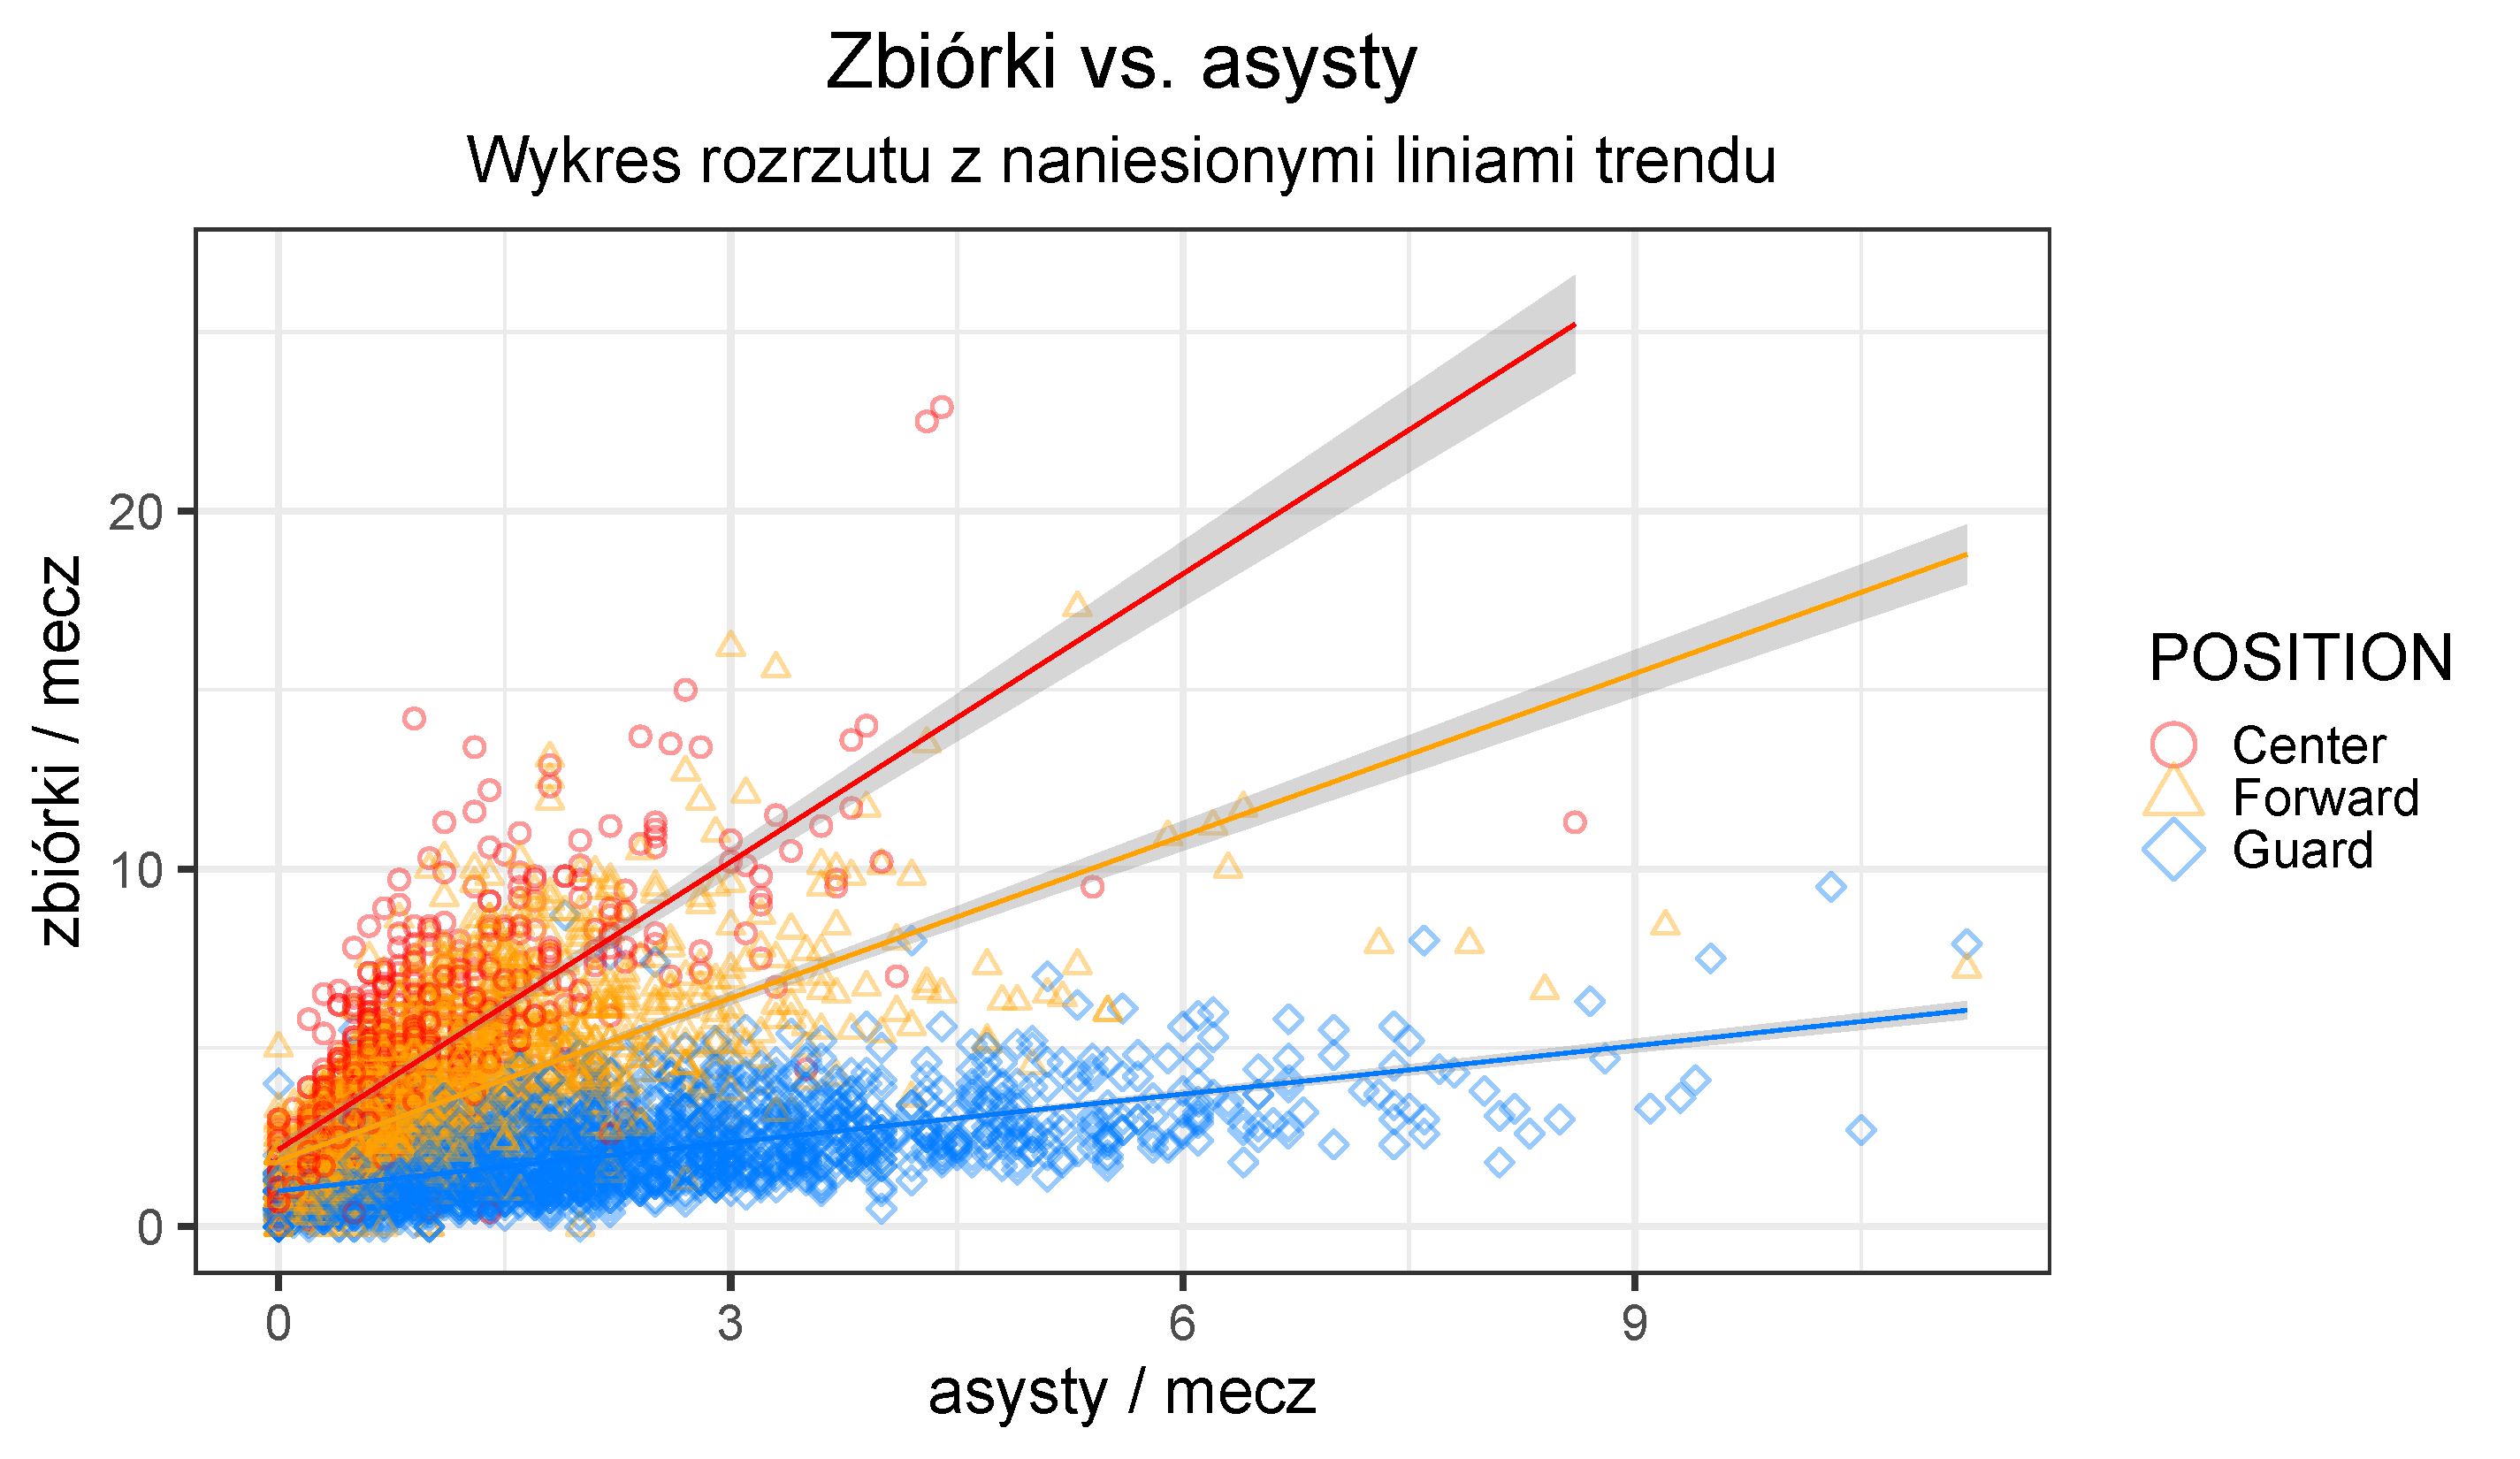
\includegraphics[width=\maxwidth]{figure/unnamed-chunk-1-1} 

}

\caption[podpis rysunku]{podpis rysunku}\label{fig:unnamed-chunk-1}
\end{figure}

\end{knitrout}

\begin{knitrout}
\definecolor{shadecolor}{rgb}{0.969, 0.969, 0.969}\color{fgcolor}\begin{figure}

{\centering 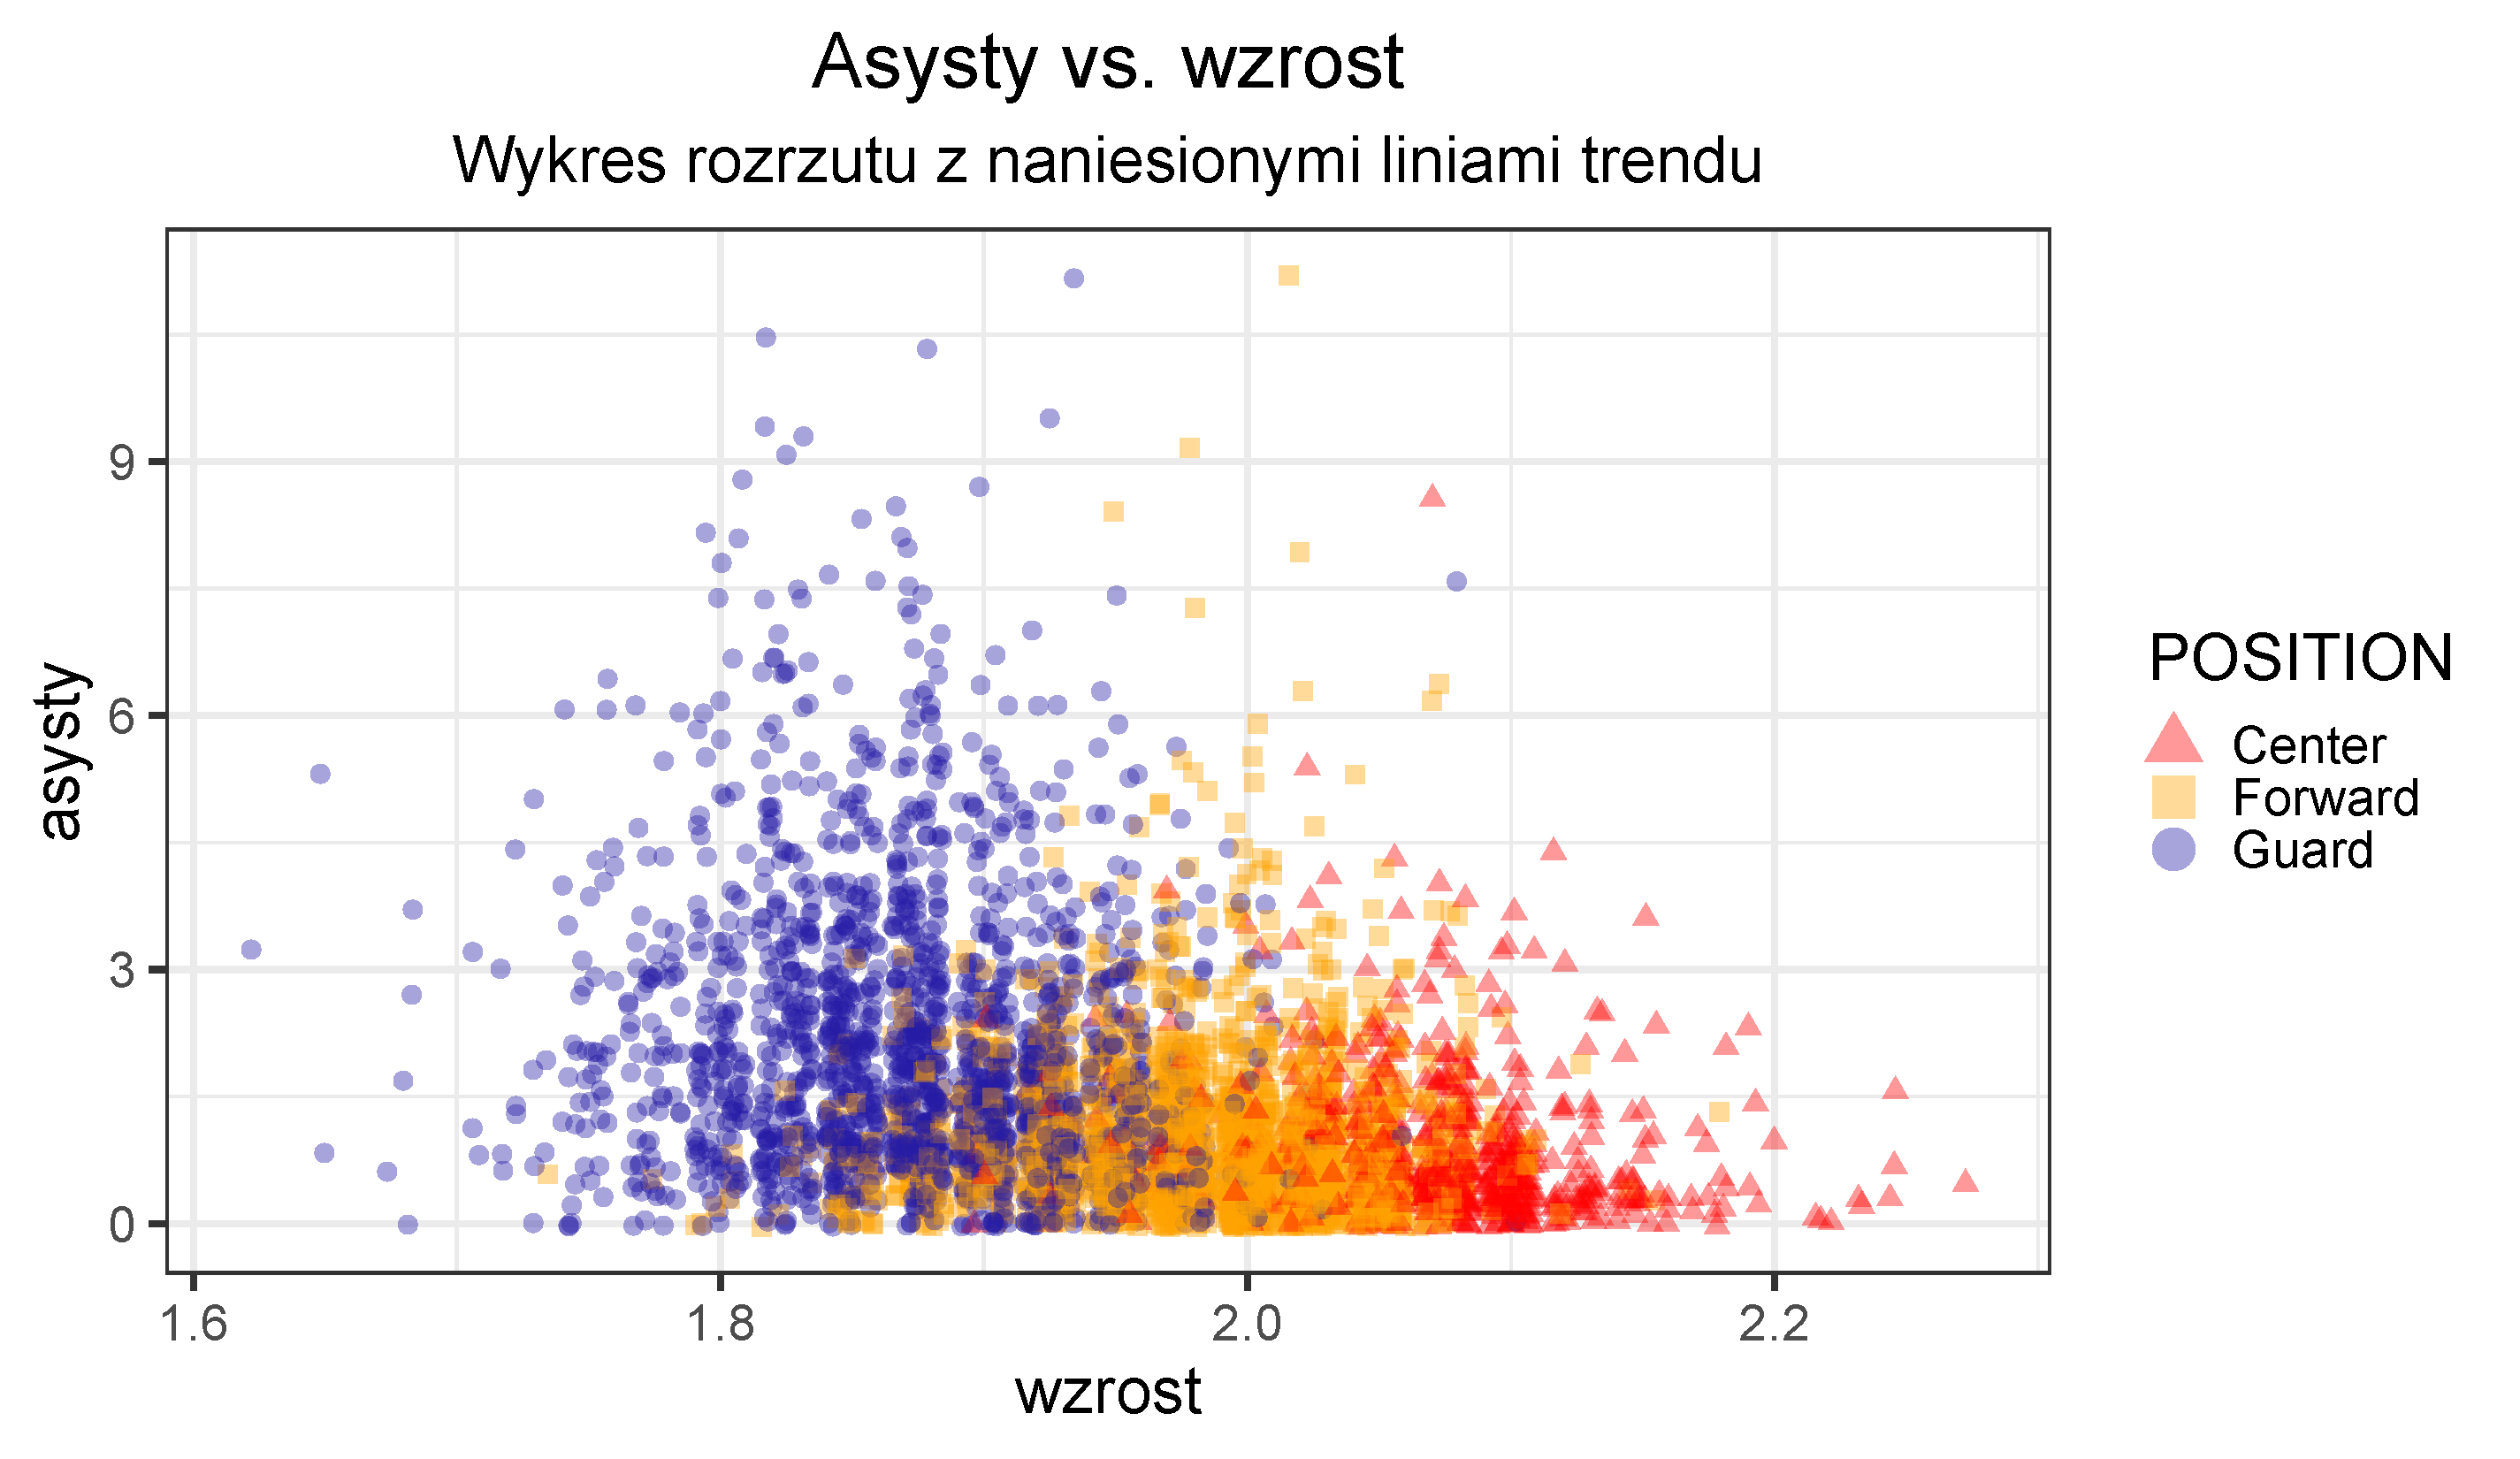
\includegraphics[width=\maxwidth]{figure/unnamed-chunk-2-1} 

}

\caption[podpis rysunku]{podpis rysunku}\label{fig:unnamed-chunk-2}
\end{figure}

\end{knitrout}

\begin{knitrout}
\definecolor{shadecolor}{rgb}{0.969, 0.969, 0.969}\color{fgcolor}\begin{figure}

{\centering 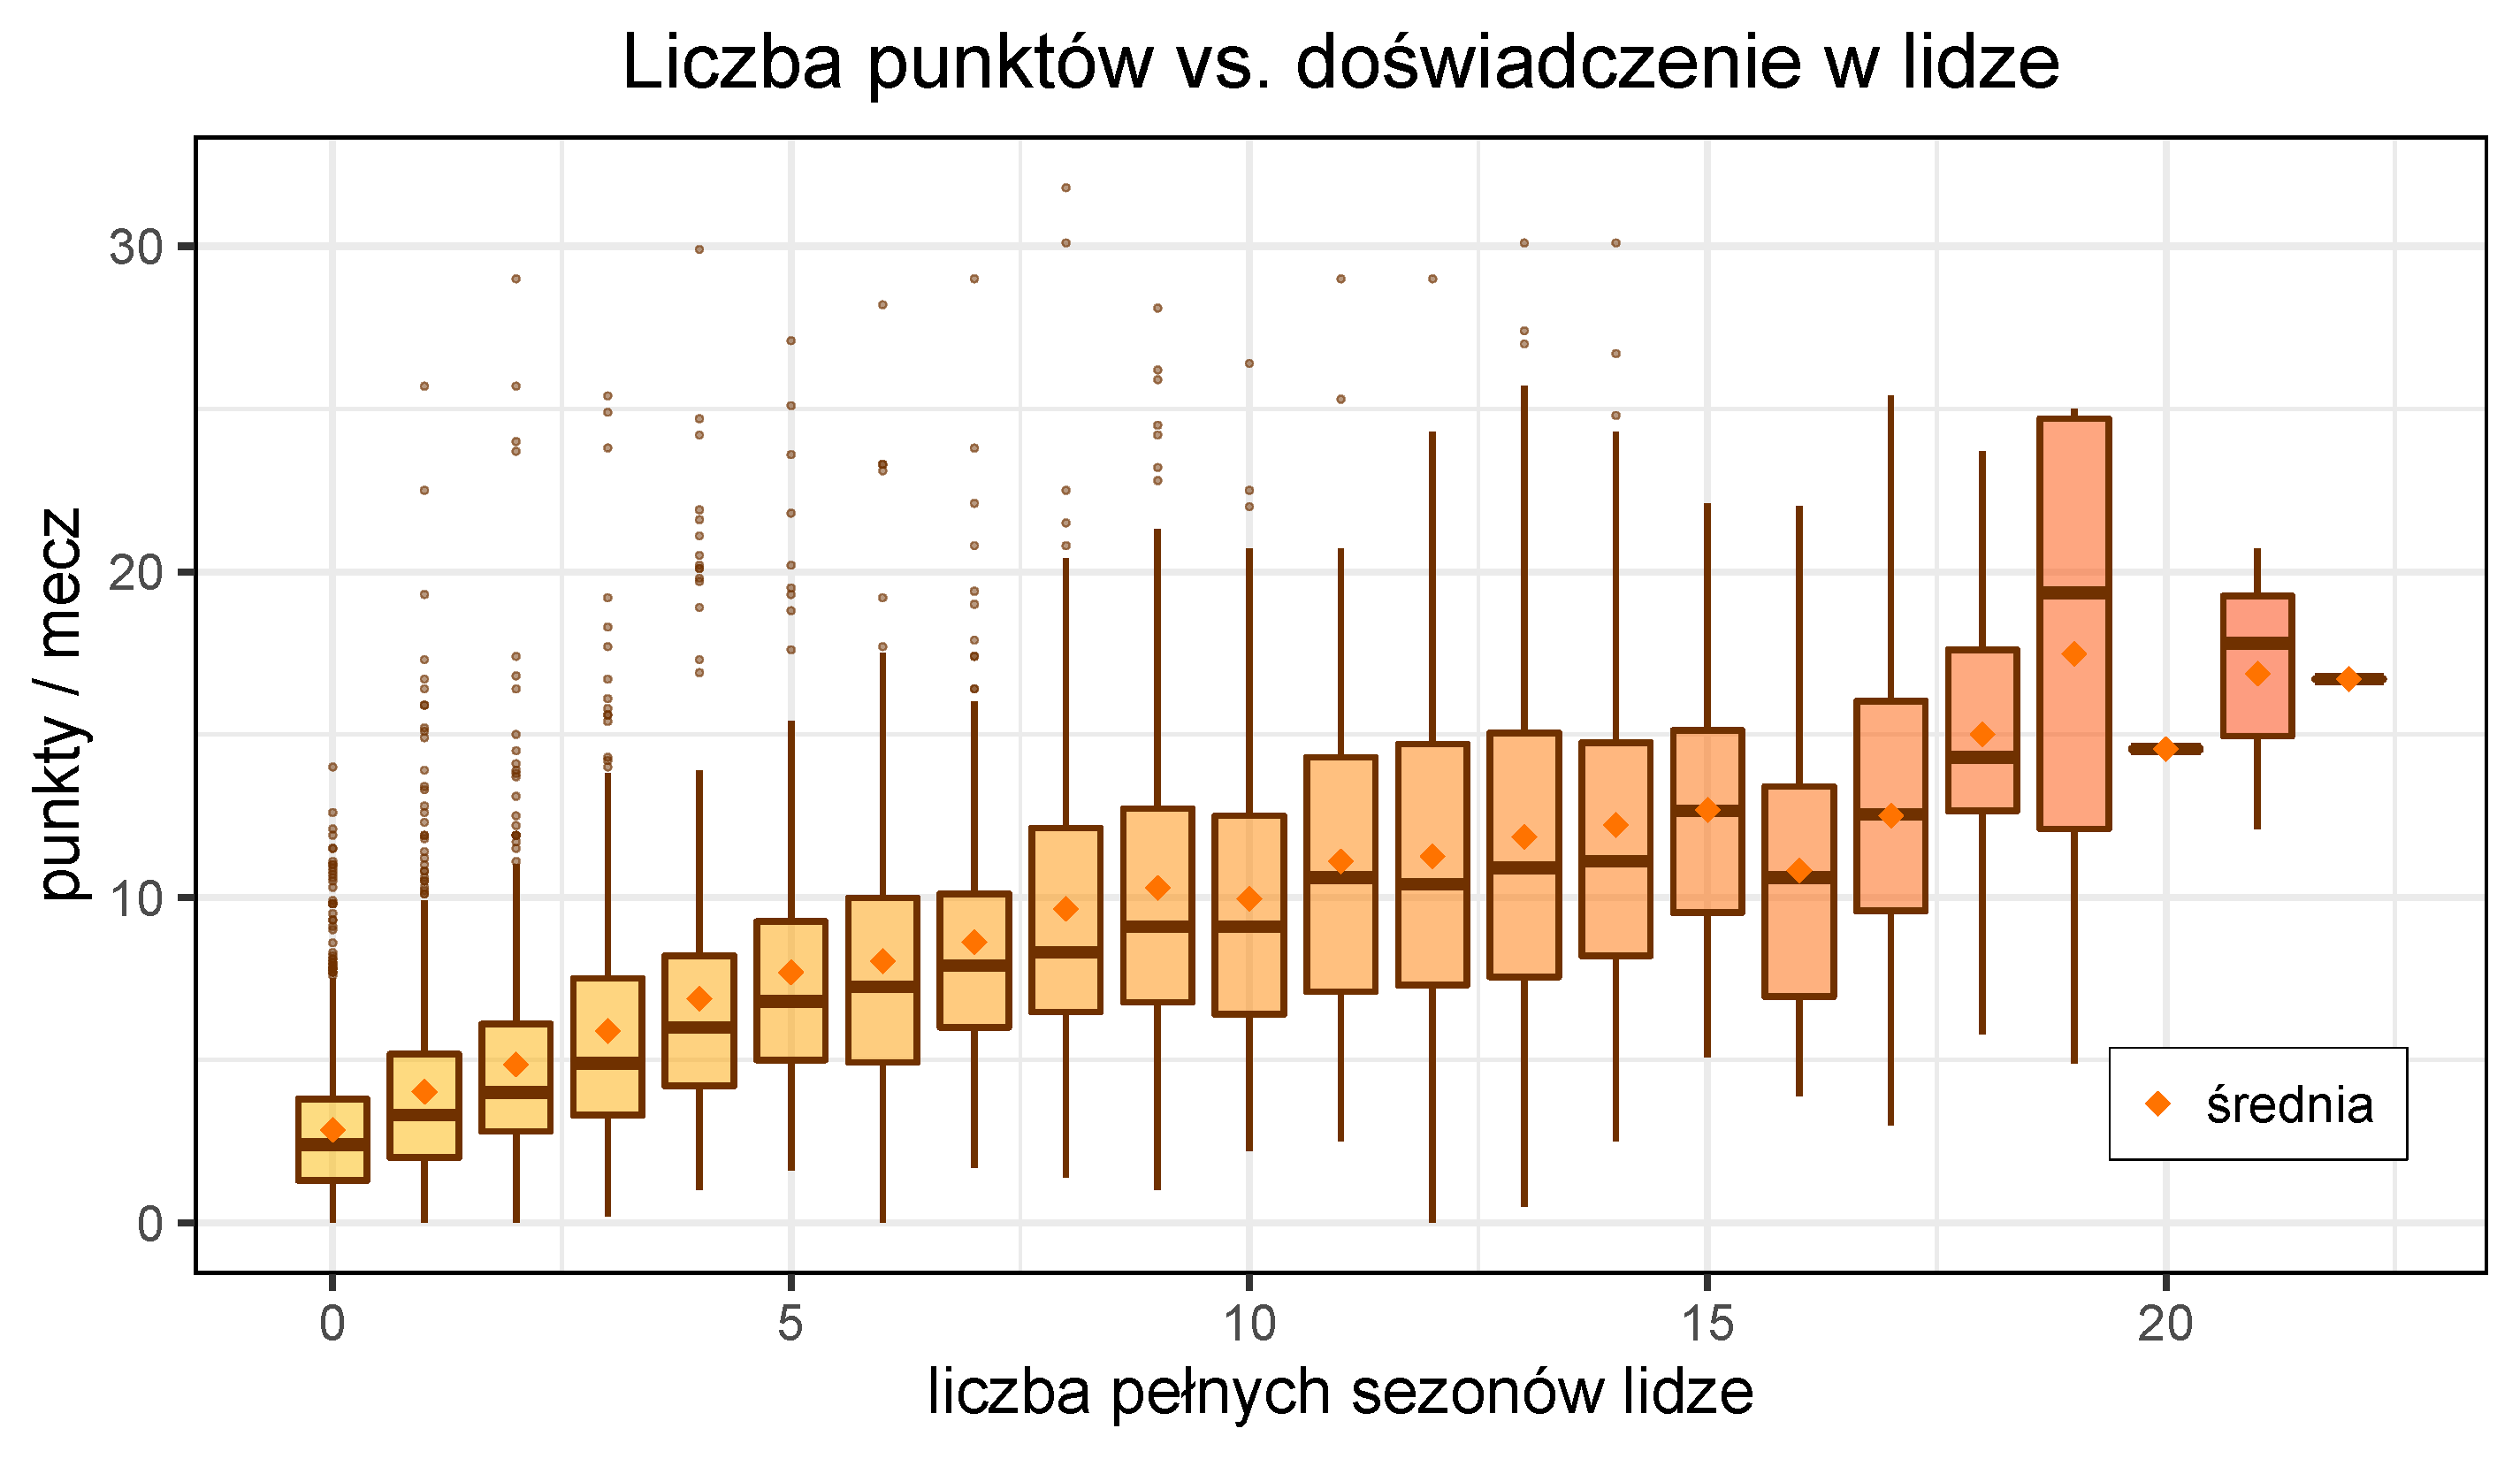
\includegraphics[width=\maxwidth]{figure/unnamed-chunk-3-1} 

}

\caption[Komentarz]{Komentarz: tylko dwóch zawodników rozegrało dokładnie 20 pełnych sezonów w lidze (Jamal Crawford i Robert Parish) i tylko jeden zawodnik rozegrał dokładnie 22 pełne sezony (Vince Carter).}\label{fig:unnamed-chunk-3}
\end{figure}

\end{knitrout}

\end{document}
